\chapter{Visualising}
\label{chapter:visualising}

\section{Displaying data within a string}

Python allows you to format a string with variables. When a variable is placed inside curly brackets \code{{}} in a formatted string (\code{f"???"}), the contents of the variable are rendered as a string. The pattern used for reading and writing files uses formatted strings:

\begin{pycode}
    file_path = "data/"
    file_name = "my_file.txt"
    formatted_string = f"{file_path}{file_name}
    print(formatted_string)
    # displays: 'data/my_file.txt'
\end{pycode}

Numerical values can be modified for display purposes by adding a formatter following a colon directly after the variable name:

Rounding formatter:

\begin{pycode}
    pi = 3.1415926
    f"The value of pi is {pi:.2} (accurate to 2 decimal places)"
    # displays: 'The value of pi is 3.14 (accurate to 2 decimal places)'
\end{pycode}

Percent formatter:

\begin{pycode}
    ratio = 0.3456
    f"Ratio as a percent is {ratio:.1%} (1 decimal place)"
    # displays: 'Ratio as a percent is 34.6% (1 decimal place)'
\end{pycode}

Comma formatter:

\begin{pycode}
    population = 2416327
    f"Current population: {population:,}"
    # displays: 'Current population: 2,416,327
\end{pycode}

\section{Simple dataframe plots}

One of the simplest ways of visualising data that is in a pandas dataframe is just to call the \code{plot()} method of the dataframe.

To see how this works, we first need to create a dataframe.

\begin{pycode}
    import pandas as pd
    data = {"city":['Brisbane','Sydney','Christchurch','Singapore','Los Angeles'],
    "rating":[4.5,4.2,4.7,4.3,3.9]}
    df = pd.DataFrame(data).set_index('city')
    print(df)
\end{pycode}

\begin{verbatim}
    city          rating
    Brisbane         4.5
    Sydney           4.2
    Christchurch     4.7
    Singapore        4.3
    Los Angeles      3.9
\end{verbatim}


\begin{pycode}
    chart = df.plot(kind='bar')
\end{pycode}

\begin{figure}[!h]
    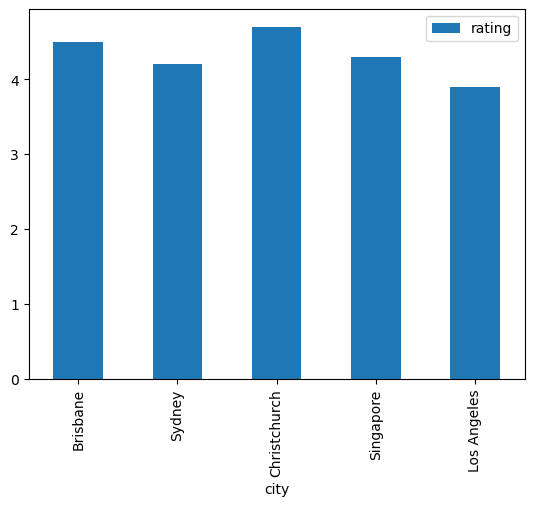
\includegraphics[width=0.5\textwidth]{graphics/simple_bar.png}
\end{figure}

\section{Charts with Plotly}

Import the relevant plotly library:

\begin{pycode}
    # import the plotly express library
    import plotly.express as px
\end{pycode}

\subsection{Box plots}

Simple box plot:

\begin{pycode}
    fig = px.box(df,x='col1')
    fig.show()
\end{pycode}

Multiple box plots based on categorical data:

\begin{pycode}
    fig = px.box(df,x='col1',color='categorical_col')
    fig.show()
\end{pycode}

\subsection{Histogram}

Simple histogram:

\begin{pycode}
    fig = px.histogram(df['col'])
    fig.show()
\end{pycode}

Specify number of bins, add a boxplot, and label the counts:

\begin{pycode}
    fig = px.histogram(df['col'],nbins=5,marginal="box",text_auto=True)
    fig.show()
\end{pycode}

Show multiple columns as a stacked histogram with color set by categorical data:

\begin{pycode}
    fig = px.histogram(df[['col1','col2']],nbins=5,marginal="box",text_auto=True,color="categorical_column")
    fig.show()
\end{pycode}
